% Left: bisection for x^3-2x-1 on [1,2.2]. Right: Rolle for x^3-3x on [0,sqrt3]. Generated by figs_t0c05.py.
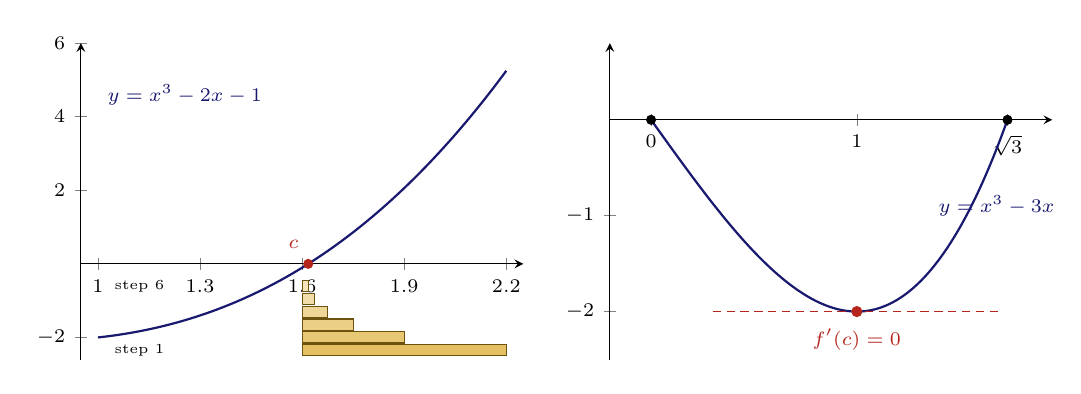
\begin{tikzpicture}
\begin{axis}[name=L,width=7.2cm,height=5.6cm,xmin=0.95,xmax=2.25,ymin=-2.6,ymax=6,axis lines=left,axis x line=middle,xtick={1,1.3,1.6,1.9,2.2},ytick={-2,2,4,6},tick label style={font=\scriptsize},clip=false]
\fill[Goldenrod!70] (axis cs:1.6000,-2.500) rectangle (axis cs:2.2000,-2.200);
\draw[Goldenrod!50!black,thin] (axis cs:1.6000,-2.500) rectangle (axis cs:2.2000,-2.200);
\fill[Goldenrod!62] (axis cs:1.6000,-2.150) rectangle (axis cs:1.9000,-1.850);
\draw[Goldenrod!50!black,thin] (axis cs:1.6000,-2.150) rectangle (axis cs:1.9000,-1.850);
\fill[Goldenrod!54] (axis cs:1.6000,-1.800) rectangle (axis cs:1.7500,-1.500);
\draw[Goldenrod!50!black,thin] (axis cs:1.6000,-1.800) rectangle (axis cs:1.7500,-1.500);
\fill[Goldenrod!46] (axis cs:1.6000,-1.450) rectangle (axis cs:1.6750,-1.150);
\draw[Goldenrod!50!black,thin] (axis cs:1.6000,-1.450) rectangle (axis cs:1.6750,-1.150);
\fill[Goldenrod!38] (axis cs:1.6000,-1.100) rectangle (axis cs:1.6375,-0.800);
\draw[Goldenrod!50!black,thin] (axis cs:1.6000,-1.100) rectangle (axis cs:1.6375,-0.800);
\fill[Goldenrod!30] (axis cs:1.6000,-0.750) rectangle (axis cs:1.6188,-0.450);
\draw[Goldenrod!50!black,thin] (axis cs:1.6000,-0.750) rectangle (axis cs:1.6188,-0.450);
\addplot[MidnightBlue,thick] coordinates {(1.0000,-2.0000) (1.0120,-1.9876) (1.0240,-1.9743) (1.0360,-1.9601) (1.0480,-1.9450) (1.0600,-1.9290) (1.0720,-1.9121) (1.0840,-1.8942) (1.0960,-1.8755) (1.1080,-1.8557) (1.1200,-1.8351) (1.1320,-1.8134) (1.1440,-1.7908) (1.1560,-1.7672) (1.1680,-1.7426) (1.1800,-1.7170) (1.1920,-1.6903) (1.2040,-1.6627) (1.2160,-1.6340) (1.2280,-1.6042) (1.2400,-1.5734) (1.2520,-1.5415) (1.2640,-1.5085) (1.2760,-1.4744) (1.2880,-1.4393) (1.3000,-1.4030) (1.3120,-1.3656) (1.3240,-1.3271) (1.3360,-1.2874) (1.3480,-1.2465) (1.3600,-1.2045) (1.3720,-1.1614) (1.3840,-1.1170) (1.3960,-1.0715) (1.4080,-1.0247) (1.4200,-0.9767) (1.4320,-0.9275) (1.4440,-0.8771) (1.4560,-0.8254) (1.4680,-0.7724) (1.4800,-0.7182) (1.4920,-0.6627) (1.5040,-0.6059) (1.5160,-0.5478) (1.5280,-0.4885) (1.5400,-0.4277) (1.5520,-0.3657) (1.5640,-0.3023) (1.5760,-0.2376) (1.5880,-0.1715) (1.6000,-0.1040) (1.6120,-0.0351) (1.6240,0.0351) (1.6360,0.1067) (1.6480,0.1798) (1.6600,0.2543) (1.6720,0.3302) (1.6840,0.4076) (1.6960,0.4864) (1.7080,0.5667) (1.7200,0.6484) (1.7320,0.7317) (1.7440,0.8164) (1.7560,0.9027) (1.7680,0.9905) (1.7800,1.0798) (1.7920,1.1706) (1.8040,1.2630) (1.8160,1.3569) (1.8280,1.4524) (1.8400,1.5495) (1.8520,1.6482) (1.8640,1.7485) (1.8760,1.8503) (1.8880,1.9539) (1.9000,2.0590) (1.9120,2.1658) (1.9240,2.2742) (1.9360,2.3843) (1.9480,2.4961) (1.9600,2.6095) (1.9720,2.7247) (1.9840,2.8415) (1.9960,2.9601) (2.0080,3.0804) (2.0200,3.2024) (2.0320,3.3262) (2.0440,3.4517) (2.0560,3.5790) (2.0680,3.7081) (2.0800,3.8389) (2.0920,3.9716) (2.1040,4.1060) (2.1160,4.2423) (2.1280,4.3804) (2.1400,4.5203) (2.1520,4.6621) (2.1640,4.8058) (2.1760,4.9513) (2.1880,5.0987) (2.2000,5.2480)};
\addplot[only marks,mark=*,mark size=1.6pt,BrickRed] coordinates {(1.6180,0)};
\node[font=\scriptsize,BrickRed,anchor=south east] at (axis cs:1.6180,0.15) {$c$};
\node[font=\scriptsize,MidnightBlue,anchor=west] at (axis cs:1.0,4.6) {$y=x^3-2x-1$};
\node[font=\tiny,anchor=west] at (axis cs:1.02,-2.35) {step $1$};
\node[font=\tiny,anchor=west] at (axis cs:1.02,-0.6) {step $6$};
\end{axis}
\begin{axis}[at={(L.east)},anchor=west,xshift=1.1cm,width=7.2cm,height=5.6cm,xmin=-0.2,xmax=1.95,ymin=-2.5,ymax=0.8,axis lines=left,axis x line=middle,xtick={0,1,1.732},xticklabels={$0$,$1$,$\sqrt3$},ytick={-2,-1},tick label style={font=\scriptsize}]
\addplot[MidnightBlue,thick] coordinates {(0.0000,0.0000) (0.0173,-0.0520) (0.0346,-0.1039) (0.0520,-0.1557) (0.0693,-0.2075) (0.0866,-0.2592) (0.1039,-0.3106) (0.1212,-0.3619) (0.1386,-0.4130) (0.1559,-0.4639) (0.1732,-0.5144) (0.1905,-0.5647) (0.2078,-0.6146) (0.2252,-0.6641) (0.2425,-0.7132) (0.2598,-0.7619) (0.2771,-0.8101) (0.2944,-0.8578) (0.3118,-0.9050) (0.3291,-0.9516) (0.3464,-0.9977) (0.3637,-1.0431) (0.3811,-1.0878) (0.3984,-1.1319) (0.4157,-1.1752) (0.4330,-1.2178) (0.4503,-1.2597) (0.4677,-1.3007) (0.4850,-1.3409) (0.5023,-1.3802) (0.5196,-1.4185) (0.5369,-1.4560) (0.5543,-1.4925) (0.5716,-1.5280) (0.5889,-1.5625) (0.6062,-1.5959) (0.6235,-1.6282) (0.6409,-1.6594) (0.6582,-1.6894) (0.6755,-1.7183) (0.6928,-1.7459) (0.7101,-1.7723) (0.7275,-1.7974) (0.7448,-1.8212) (0.7621,-1.8437) (0.7794,-1.8648) (0.7967,-1.8845) (0.8141,-1.9027) (0.8314,-1.9195) (0.8487,-1.9348) (0.8660,-1.9486) (0.8833,-1.9608) (0.9007,-1.9714) (0.9180,-1.9804) (0.9353,-1.9877) (0.9526,-1.9934) (0.9699,-1.9973) (0.9873,-1.9995) (1.0046,-1.9999) (1.0219,-1.9985) (1.0392,-1.9953) (1.0566,-1.9902) (1.0739,-1.9832) (1.0912,-1.9743) (1.1085,-1.9634) (1.1258,-1.9505) (1.1432,-1.9356) (1.1605,-1.9186) (1.1778,-1.8995) (1.1951,-1.8784) (1.2124,-1.8550) (1.2298,-1.8295) (1.2471,-1.8018) (1.2644,-1.7718) (1.2817,-1.7395) (1.2990,-1.7050) (1.3164,-1.6681) (1.3337,-1.6288) (1.3510,-1.5872) (1.3683,-1.5431) (1.3856,-1.4965) (1.4030,-1.4474) (1.4203,-1.3959) (1.4376,-1.3417) (1.4549,-1.2850) (1.4722,-1.2256) (1.4896,-1.1636) (1.5069,-1.0990) (1.5242,-1.0316) (1.5415,-0.9614) (1.5588,-0.8885) (1.5762,-0.8128) (1.5935,-0.7343) (1.6108,-0.6529) (1.6281,-0.5685) (1.6454,-0.4813) (1.6628,-0.3911) (1.6801,-0.2979) (1.6974,-0.2017) (1.7147,-0.1024) (1.7321,-0.0000)};
\addplot[BrickRed,densely dashed] coordinates {(0.3,-2) (1.7,-2)};
\addplot[only marks,mark=*,mark size=1.6pt,black] coordinates {(0,0) (1.7321,0)};
\addplot[only marks,mark=*,mark size=1.8pt,BrickRed] coordinates {(1,-2)};
\node[font=\scriptsize,BrickRed,anchor=north] at (axis cs:1,-2.08) {$f'(c)=0$};
\node[font=\scriptsize,MidnightBlue,anchor=west] at (axis cs:1.35,-0.9) {$y=x^3-3x$};
\end{axis}
\end{tikzpicture}
